% Options for packages loaded elsewhere
\PassOptionsToPackage{unicode}{hyperref}
\PassOptionsToPackage{hyphens}{url}
%
\documentclass[
]{article}
\author{}
\date{\vspace{-2.5em}}

\usepackage{amsmath,amssymb}
\usepackage{lmodern}
\usepackage{iftex}
\ifPDFTeX
  \usepackage[T1]{fontenc}
  \usepackage[utf8]{inputenc}
  \usepackage{textcomp} % provide euro and other symbols
\else % if luatex or xetex
  \usepackage{unicode-math}
  \defaultfontfeatures{Scale=MatchLowercase}
  \defaultfontfeatures[\rmfamily]{Ligatures=TeX,Scale=1}
\fi
% Use upquote if available, for straight quotes in verbatim environments
\IfFileExists{upquote.sty}{\usepackage{upquote}}{}
\IfFileExists{microtype.sty}{% use microtype if available
  \usepackage[]{microtype}
  \UseMicrotypeSet[protrusion]{basicmath} % disable protrusion for tt fonts
}{}
\makeatletter
\@ifundefined{KOMAClassName}{% if non-KOMA class
  \IfFileExists{parskip.sty}{%
    \usepackage{parskip}
  }{% else
    \setlength{\parindent}{0pt}
    \setlength{\parskip}{6pt plus 2pt minus 1pt}}
}{% if KOMA class
  \KOMAoptions{parskip=half}}
\makeatother
\usepackage{xcolor}
\IfFileExists{xurl.sty}{\usepackage{xurl}}{} % add URL line breaks if available
\IfFileExists{bookmark.sty}{\usepackage{bookmark}}{\usepackage{hyperref}}
\hypersetup{
  hidelinks,
  pdfcreator={LaTeX via pandoc}}
\urlstyle{same} % disable monospaced font for URLs
\usepackage[margin=1in]{geometry}
\usepackage{graphicx}
\makeatletter
\def\maxwidth{\ifdim\Gin@nat@width>\linewidth\linewidth\else\Gin@nat@width\fi}
\def\maxheight{\ifdim\Gin@nat@height>\textheight\textheight\else\Gin@nat@height\fi}
\makeatother
% Scale images if necessary, so that they will not overflow the page
% margins by default, and it is still possible to overwrite the defaults
% using explicit options in \includegraphics[width, height, ...]{}
\setkeys{Gin}{width=\maxwidth,height=\maxheight,keepaspectratio}
% Set default figure placement to htbp
\makeatletter
\def\fps@figure{htbp}
\makeatother
\setlength{\emergencystretch}{3em} % prevent overfull lines
\providecommand{\tightlist}{%
  \setlength{\itemsep}{0pt}\setlength{\parskip}{0pt}}
\setcounter{secnumdepth}{-\maxdimen} % remove section numbering
\ifLuaTeX
  \usepackage{selnolig}  % disable illegal ligatures
\fi

\begin{document}

\hypertarget{species-status-assessment}{%
\section{Species Status Assessment}\label{species-status-assessment}}

\hypertarget{species-name-pineneedle-milkweed-asclepias-linaria}{%
\subsection{\texorpdfstring{Species Name: Pineneedle milkweed
\emph{Asclepias
linaria}}{Species Name: Pineneedle milkweed Asclepias linaria}}\label{species-name-pineneedle-milkweed-asclepias-linaria}}

\hypertarget{species-taxonomy-taxon-key-3170270}{%
\subsection{Species Taxonomy: Taxon key
3170270}\label{species-taxonomy-taxon-key-3170270}}

\hypertarget{species-description}{%
\subsection{Species Description:}\label{species-description}}

\emph{A. linaria} is a rare milkweed species in the US, but common and
found throughout Mexico. It can grow up to 4 feet tall, but is typically
around 2 feet tall. It flowers in the spring and summer annually. It has
small, white flowers, woody stems, and needle-shaped leaves.

\hypertarget{habitat-description}{%
\subsection{Habitat Description:}\label{habitat-description}}

\begin{itemize}
\tightlist
\item
  Dry rocky slopes and mesas
\item
  elevation: 1500-6000ft
\end{itemize}

\hypertarget{larval-host-information}{%
\subsection{Larval Host Information:}\label{larval-host-information}}

It is known to be a host plant for monarch butterflies and other
pollinators. However, it is used only occassionally due to its relative
toxicity.

\hypertarget{data-sources-for-occurence-and-distribution-modeling}{%
\subsection{Data Sources for Occurence and Distribution
Modeling:}\label{data-sources-for-occurence-and-distribution-modeling}}

\begin{itemize}
\tightlist
\item
  GBIF
\item
  iNaturalist
\end{itemize}

\hypertarget{species-occurence-map}{%
\subsection{Species Occurence Map:}\label{species-occurence-map}}

\begin{figure}
\centering
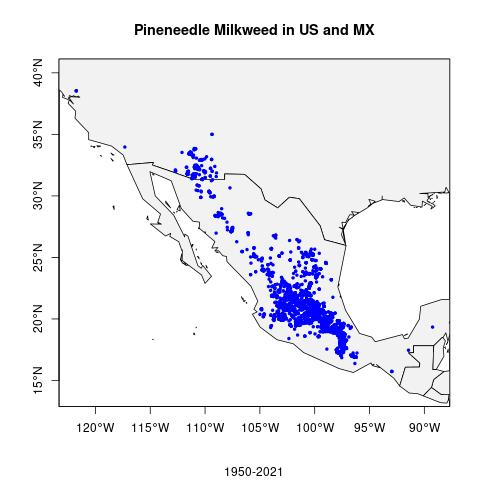
\includegraphics{images/MUSMXspocc.jpg}
\caption{Map}
\end{figure}

Link to GitHub Repository:

\href{mapping.Rmd}{Mapping}

References:

Nabhan, G., S. Buckley, and H. Dial. 2015. Pollinator Plants of the
Desert Southwest: Native Milkweeds (Asclepias spp.). USDA-Natural
Resources Conservation Service, Tucson Plant Materials Center, Tucson,
AZ. TN-PM-16-1-AZ.

\end{document}
